\documentclass[twocolumn]{article}
\usepackage{graphicx}
\usepackage{amsmath}
\usepackage{amssymb} %Use of therefore symbol
\usepackage{hyperref}
\usepackage{caption}



\begin{document}
\title{Lab 1: Monte Carlo Methods}
\author{Alex Matheson, Austin Nguyen}
%\affiliation{Department of Physics and Astronomy, University of Calgary, Calgary AB T2N 1N4 Canada}
\date{\today}
\maketitle

\section{Introduction}

\section{Methods}
\subsection{Random Numbers}
Fortran code was written to generate random numbers using a pseudo-random number generator, using input parameters $I_0=3$, $A=7$, $C=0$, and $M=10$. The sequence was shown to repeat, following a pattern of $1,7,9,3,...$ . This pattern is clearly not random, and repeats. The sequence must repeat after at most $M$ entries. Since there are $M$ possible results from the equation, the longest possible sequence generates each number $0=<n<M$ at most once, since once a previous value from the sequence is drawn, the sequence begins to repeat. 

A more elaborate version of this pseudo-random generator was constructed with larger constants. A correlation plot was made to visualize how subsequent values in the sequence were related. Figure \ref{fig:fig1} shows the plot. The result shows that this sequence is not truly random, with some pattern existing between the subsequent numbers. For a 'truly random' sequence, some numbers might be more related than others, and it would be expected that while all numbers did not have the same correlation, at least some would. Another correlation plot, figure \ref{fig:fig2}, shows a different problem. The numbers in the sequence clearly follow a repeating pattern. Figure \ref{fig:fig3} shows a plot without such problems. The results in this case appear to have no correlation between $x_n$ and $x_{n+1}$ and are shown similar to random noise.

\begin{figure}
\centering
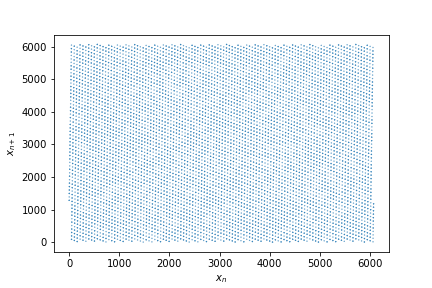
\includegraphics[width=0.7\linewidth]{fig1}
\caption{A correlation plot for a pseudo-random sequence with $A=106$, $C=1283$, and $M=6075$.}
\label{fig:fig1}
\end{figure}

\begin{figure}
	\centering
	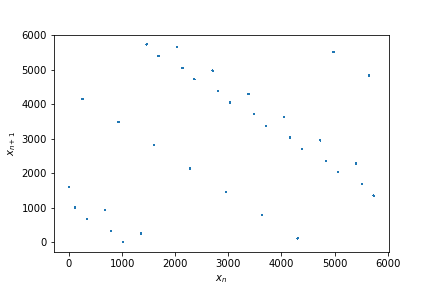
\includegraphics[width=0.7\linewidth]{fig2}
	\caption{A correlation plot for a pseudo-random sequence with $A=107$, $C=1283$, and $M=6075$. Note that this is a change of 1 in variable $A$ from figure \ref{fig:fig2}}
	\label{fig:fig2}
\end{figure}

\begin{figure}
	\centering
	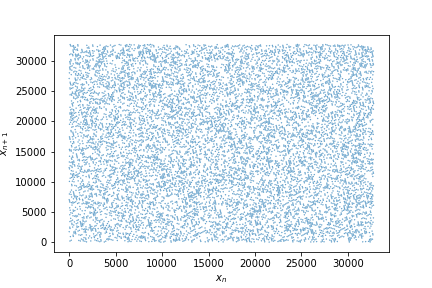
\includegraphics[width=0.7\linewidth]{fig3}
	\caption{A correlation plot for a pseudo-random sequence with $A=1103515245$, $C=12345$, and $M=32768$.}
	\label{fig:fig3}
\end{figure}

Next, the autocorrelation function was examined. A good sequence of random numbers should have a low autocorrelation value. The above pseudo-random generator was tested alongside the gfortran random number generator.

\begin{figure}
\centering
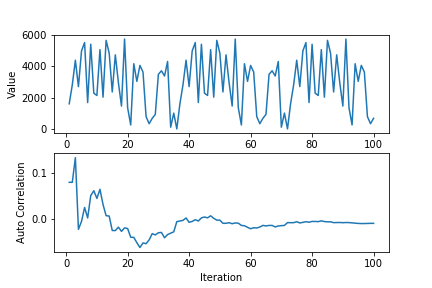
\includegraphics[width=0.7\linewidth]{fig4}
\caption{Random numbers generated by the same pseudo-random generator as figure \ref{fig:fig3}. The top plot shows the numbers generated, while the bottom plot shows the auto-correlation function.}
\label{fig:fig4}
\end{figure}

\begin{figure}
	\centering
	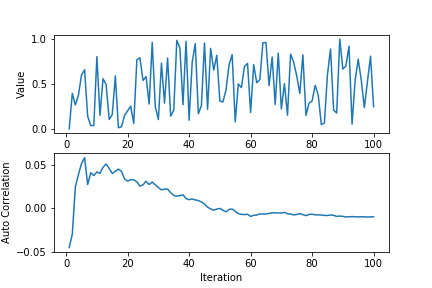
\includegraphics[width=0.7\linewidth]{fig5}
	\caption{Random numbers generated by gfortran's internal RAND() function.}
	\label{fig:fig4}
\end{figure}

\subsection{Light Diffusion}
A number of equations were provided for different parameters in a light diffusion scenario. In this scenario, a photon enters a uniform slab and interacts with matter inside. The possible interactions are absorption, scattering, or exiting the medium. To simulate the path of a single photon through the slab, each parameter in the equations need to be randomly sampled. These parameters are not necessarily uniform. First, a sampling equation for optical depth was determined:
\begin{equation}
\begin{split}
P(\tau) d\tau =& e^{-\tau} d\tau \\
\therefore F_{\tau}(\tau) =& e^{-\tau} \\
\tau =& F^{-1}_{\tau}(u) \\
\tau =& e^{u}
\end{split}
\end{equation}

Next, the distribution for initial orientation $\theta$ was provided. From this random samples could be determined:
\begin{equation}
\begin{split}
P(\theta) d\theta =& \frac{1}{2} \sin(\theta) \\
\therefore F_{\theta}(\theta) =& \frac{1}{2} \sin(\theta)\\
\theta =& F^{-1}_{\theta}(u) \\
\theta =& \sin^{-1}(2u)
\end{split}
\end{equation}

Lastly, angle $\phi$ needed to be considered. Thankfully, this variable was already uniform.

The length travelled through the medium was dependent on the optical depth.
\begin{equation}
\begin{split}
L =& \int_{0}^{\tau_{max}}\sigma n dz \\
\end{split}
\end{equation}

For most of the path of a photon, the exit condition will not be in play. For the rest of the medium, the probability of a photon being scattered is:
\begin{equation}
prob = \frac{P_s}{P_s + P_a}
\end{equation}

Since the two probabilities must add together to $1$, the absorb or scatter condition has value $1$ associated with complete scattering (when $P_s = 1$ and $P_a=0$) or value $0$ for complete absorption (when $P_s = 0$ and $P_a=1$).

\subsection{Annealing}
In an annealing procedure, the acceptance probability of completing a change after a proposed step forward is modified by a temperature $T$. The acceptance is now defined as:
$A(x_n \to x^*) = Min \Bigg( 1, \Big( \frac{P(x^*)}{P(x_n)}\Big) ^{ \frac{1}{T(n)} } \Bigg)$
When $T=1$, the algorithm that is recovered is a simple metropolis algorithm. 

In a hyporthetical scenario, the probability term is set to 0.5 and $T=100$ initially, yielding acceptance of $0.93$. After some time, $T=1$ and the acceptance reduces to $0.5$. After still more time, $T=0.1$ and the acceptance is $0.000977$. Because of the inverse nature of $T$ in the exponent, a reduction in $T$ makes a change exponentially less likely to occur. This is typically desirable when using annealing. Ideally, the random walker being used by the algorithm is able to escape local maxima and jump to other peaks in the region early on. As time goes on, the algorithm should lower the acceptance so that it hones in on the actual peak.

%Seek clarification on e^-E question

\section{Discussion}


\section{Conclusion}

\begin{thebibliography}{00}
	\bibitem{ouyed}
	Ouyed and Dobler, PHYS 581 course notes, Department of Physics and Astrophysics, University of Calgary (2016).
	\bibitem{NR}
	W. Press et al., \emph{Numerical Recipes} (Cambridge University Press, 2010) 2nd. Ed.
\end{thebibliography}

\section{Appendix}

	
\end{document}